%%%%%%%%%%%%%%%%%%%%%%%%%%%%%%%%%%%%%%%%%%%%%%%%%%%%%%%%%%%%%%%%%%%%%%%%%%%%%%%%
%% MASTER'S THESIS                                                            %%
%%                                                                            %% 
%% Title (en): Multi-Agent Systems and Organizations                          %%
%% Title (cs): Multiagentní systémy a organizace                              %%
%%                                                                            %%
%% Author: Bc. Lukáš Kúdela                                                   %%
%% Supervisor: Prof. RNDr. Petr Štěpánek, DrSc.                               %%
%%                                                                            %%
%% Academic year: 2011/2012                                                   %%
%%%%%%%%%%%%%%%%%%%%%%%%%%%%%%%%%%%%%%%%%%%%%%%%%%%%%%%%%%%%%%%%%%%%%%%%%%%%%%%%

\section{Example 2: Arithmetic Expression Evaluation}

% Section intro - 'Arithmetic expression evaluation' organziation
This example demonstrates a not-so-simple organization---\textit{arithmetic expression evaluation}.
% 'Arithmetic expression evaluation' - purpose
The purpose of this organization is to facilitate divide-and-conquer evaluation of arithmetic expressions by grouping five agents: one agent \textit{breaks the expression down} (the \textit{divide} part) and the other four compute \textit{addition}, \textit{subtraction}, \textit{multiplication} and \textit{integral division} (the \textit{conquer} part), each agent computing one arithmetic operation.
The reason the organization is formed in the first place is because the agent breaking the expression down is not capable of computing any arithmetic operation itself.
% Assumptions - simple arithmetic expression
In this example, agents evaluate simple arithmetic expressions---consisting of natural numbers, four basic arithmetic operations (addition, subtraction, multiplication and integral division) and parentheses. However, it should be apparent that any arithmetic expressions could be evaluated this way.

%%%%%%%%%%%%%%%%%%%%%%%%%%%%%%%%%%%%%%%%%%%%%%%%%%%%%%%%%%%%%%%%%%%%%%%%%%%%%%%%
\subsection*{Specification}

%%%%%%%%%%%%%%%%%%%%%%%%%%%%%%%%%%%%%%%%%%%%%%%%%%%%%%%%%%%%%%%%%%%%%%%%%%%%%%%%
\subsubsection*{Organization Part}

% 'Expression evaluation' organizaiton type
The \textit{Expression evaluation} organization type (modelled by the \texttt{ExpressionEvaluation\_Organization} agent class) contains five roles---\textit{Evaluator}, \textit{Adder}, \textit{Subtractor}, \textit{Multiplier} and \textit{Divider}---and two protocols---\textit{Evaluate expression} and \textit{Evaluate binary operation}.
% 'expression-evaluation' organization
\textit{Expression evaluation} has one instance in the running MAS: the \textit{expression-evaluation} organization (modelled by the \texttt{expressionEvaluation\_Organization} agent instance).

% 'Evaluator' role
The \textit{Evaluator} role (modelled by the \texttt{Evaluator\_Role} agent class) can evaluate a simple arithmetic expression.
% 'Evaluator' role - multiplicity, competences & responsibilities
The \textit{Evaluator} role is a \textit{multiple} role\footnote{However, only one agent plays the \textit{Evaluator} role in our example.}.
It has one competence---\textit{Evaluate}---and no responsibilities.

% 'Evaluate' competence
The \textit{Evaluate} competence (modelled by the \texttt{Evaluate\_Competence} class) is a competence to evaluate a simple arithmetic expression.
% 'Evaluate' competence - argument & result
It has one argument---an expression (a string)---and one result---the value of this expression (an integer).

% 'Adder' role
The \textit{Adder} role (modelled by the \texttt{Adder\_Role} agent class) can perform addition of two simple arithmetic expressions.
% 'Adder' role - multiplicity, competences & responsibilities
The \textit{Adder} role is a \textit{multiple} role\footnote{However, only one agent plays the \textit{Adder} role in our example.}.
It has no competences and one responsibility---\textit{Add}.

% 'Add' responsibility
The \textit{Add} responsibility (modelled by the \texttt{Add\_Responsibility} class) is a responsibility to perform addition of two integers.
% 'Add' responsibility - argument & result
It has two arguments---a pair of addends---and one result---their sum.

% 'Subtractor' role
The \textit{Subtractor} role (modelled by the \texttt{Subtractor\_Role} agent class) can perform subtraction of two simple arithmetic expressions.
% 'Subtractor' role - multiplicity, competences & responsibilities
The \textit{Subtractor} role is a \textit{multiple} role\footnote{However, only one agent plays the \textit{Subtractor} role in our example.}.
It has no competences and one responsibility---\textit{Subtract}.

% 'Subtract' responsibility
The \textit{Subtract} responsibility (modelled by the \texttt{Subtract\_Responsibility} class) is a responsibility to perform subtraction of two integers.
% 'Subtract' responsibility - argument & result
It has two arguments---a minuend and a subtrahend---and one result---their difference.

% 'Multiplier' role
The \textit{Multiplier} role (modelled by the \texttt{Multiplier\_Role} agent class) can perform multiplication of two simple arithmetic expressions.
% 'Multiplier' role - multiplicity, competences & responsibilities
The \textit{Multiplier} role is a \textit{multiple} role\footnote{However, only one agent plays the \textit{Multiplier} role in our example.}.
It has no competences and one responsibility---\textit{Multiply}.

% 'Multiply' responsibility
The \textit{Multiply} responsibility (modelled by the \texttt{Multiply\_Responsibility} class) is a responsibility to perform multiplication of two integers.
% 'Multiply' responsibility - argument & result
It has two arguments---a pair of factors---and one result---their product.

% 'Divider' role
The \textit{Divider} role (modelled by the \texttt{Divider\_Role} agent class) can perform division of two simple arithmetic expressions.
% 'Divider' role - multiplicity, competences & responsibilities
The \textit{Divider} role is a \textit{multiple} role\footnote{However, only one agent plays the \textit{Divider} role in our example.}.
It has no competences and one responsibility---\textit{Divide}.

% 'Divide' responsibility
The \textit{Divide} responsibility (modelled by the \texttt{Divide\_Responsibility} class) is a responsibility to perform integral division of two integers.
% 'Multiply' responsibility - argument & result
It has two arguments---a dividend and a divisor---and one result---their quotient.

% 'Binary operator' role
In the following, we will use the \textit{Binary operator} abstract role to refer to refer to the \textit{Adder}, \textit{Subtractor}, \textit{Multiplier} or \textit{Divisor} role where it is not necessary to distinguish between them.

%%%%%%%%%%%%%%%%%%%%%%%%%%%%%%%%%%%%%%%%%%%%%%%%%%%%%%%%%%%%%%%%%%%%%%%%%%%%%%%%
\subsubsection*{Protocol Part}

% 'Evaluate expresion' protocol
The \textit{Evaluate expression} protocol (modelled by the \texttt{EvaluateExpressionProtocol} class) is a protocol by which a \textit{Binary operator} (the initiator party, modelled by the \texttt{EvaluateExpression\_InitiatorParty}) requests an \textit{Evaluator} (the responder party, modelled by the \texttt{EvaluateExpression\_ResponderParty}) to evaluate an expression.

% 'Evaluate expression request' message
The \textit{Evaluate expression request} message (modelled by the \texttt{EvaluateExpressionRequestMessage} class) is a message sent by a \textit{Binary operator} to an \textit{Evaluator} requesting the latter to evaluate an expression.

% 'Evalaute expression reply' message
The \textit{Evaluate expression reply} message (modelled by the \texttt{EvaluateExpressionReplyMessage} class) is a message sent by an \textit{Evaluator} to a \textit{Binary operator} informing the latter about the value of the evaluated expression.

% 'Evaluate binary operation' protocol
The \textit{Evaluate binary operation} protocol (modelled by the \texttt{EvaluateBinaryOperationProtocol} class) is a protocol by which an \textit{Evaluator} (the initiator party, modelled by the \texttt{EvaluateBinaryOperation\_InitiatorParty}) requests a \textit{Binary operator} (the responder party, modelled by the \texttt{EvaluateBinaryOperation\_ResponderParty}) to evaluate a binary operation.

% 'Evalaute binary operation request' message
The \textit{Evaluate binary operation request} message (modelled by the \texttt{EvaluateBinaryOperationReqestMessage} class) is a message sent by a \textit{Evaluator} to a \textit{Binary Operator} requesting the latter to evaluate a binary operation between two operand expressions.

% 'Evaluate binary operation reply' message
The \textit{Evaluate binary operation reply} message (modelled by the \texttt{EvaluateBinaryOperationReplyMessage} class) is a message sent by a \textit{Binary operator} to an \textit{Evaluator} informing the latter about the value of the evaluated binary operation.

%%%%%%%%%%%%%%%%%%%%%%%%%%%%%%%%%%%%%%%%%%%%%%%%%%%%%%%%%%%%%%%%%%%%%%%%%%%%%%%%
\subsubsection*{Player Part}

% 'Blank' player type
The \textit{Blank} player type (modelled by the \texttt{Blank\_Player} agent class) is a player with no capabilities.
It has one instance in the running MAS: \textit{player1}.
% 'player1' player
\textit{player1} (modelled by the \texttt{player1} agent instance) intends to enact the \textit{Evaluator} role in the \textit{expression-evaluation} organization and to exercise the role's \textit{Evaluate} competence---to have an expression evaluated by the players of the \textit{Binary operator} roles.

% 'Addition computer' player type
The \textit{Addition computer} player type (modelled by the \texttt{AdditionComputer\_Player} agent class) is a player capable of computing the addition operation.
It has one instance in the running MAS: \textit{player2}.
% 'player2' player
\textit{player2} (modelled by the \texttt{player2} agent instance) intends to enact the \textit{Adder} role in the \textit{expression-evaluation} organization and fulfil the role's \textit{Add} responsibility---to compute addition during the evaluation of the expression from the player of the \textit{Evaluator} role.

% 'Subtraction computer' player type
The \textit{Subtraction computer} player type (modelled by the \texttt{SubtractionComputer\_Player} agent class) is a player capable of computing the subtraction operation.
It has one instance in the running MAS: \textit{player3}.
% 'player3' player
The intention of \textit{player3} (modelled by the \texttt{player3} agent instance) is to enact the \textit{Subtractor} role in the \textbf{expression-evaluation} organization and perform the role's \textit{Subtract} responsibility---to compute subtraction during the evaluation of the expression from the player of the  \textit{Evaluator} role.

% 'Multiplication computer' player type
The \textit{Multiplication computer} player type (modelled by the \texttt{MultiplicationComputer\_Player} agent class) is a player capable of computing the multiplication operation.
It has one instance in the running MAS: \textit{player4}.
% 'player4' player
\textit{player4} (modelled by the \texttt{player4} agent instance) intends to enact the \textit{Multiplier} role in the \textit{expression-evaluation} organization and fulfil the role's \textit{Multiply} responsibility---to compute multiplication during the evaluation of the expression from the player of the \textit{Evaluator} role.

% 'Division computer' player type
The \textit{Division computer} player type (modelled by the \texttt{DivisionComputer\_Player} agent class) is a player capable of computing the division operation.
It has one instance in the running MAS: \textit{player5}.
% 'player5' player
The intention of \textit{player5} (modelled by the \texttt{player5} agent instance) is to enact the \textit{Divisor} role in the \textit{expression-evaluation} organization and fulfil the role's \textit{Divide} responsibility---to compute division during the evaluation of the expression from the player of the \textit{Evaluator} role.

%%%%%%%%%%%%%%%%%%%%%%%%%%%%%%%%%%%%%%%%%%%%%%%%%%%%%%%%%%%%%%%%%%%%%%%%%%%%%%%%
\subsection*{Manifestation}

%%%%%%%%%%%%%%%%%%%%%%%%%%%%%%%%%%%%%%%%%%%%%%%%%%%%%%%%%%%%%%%%%%%%%%%%%%%%%%%%
\subsubsection*{Stage 1: Role Enactment}

% Figure: Stage 1: Role enactment
\begin{figure}[H]
	\centering
	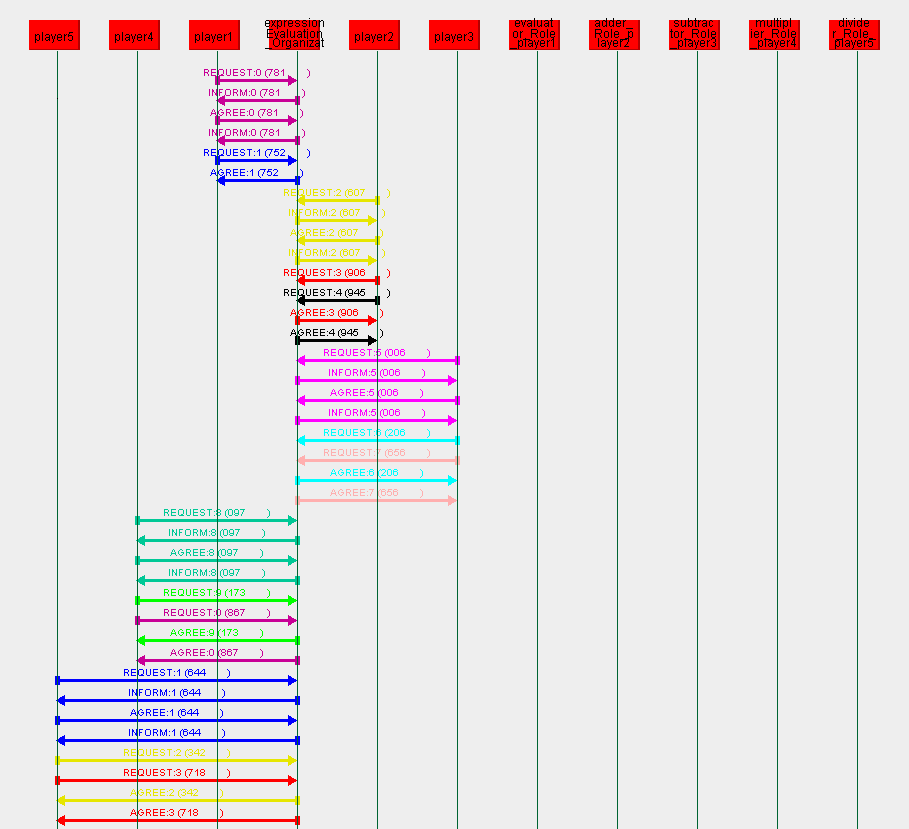
\includegraphics[width=\textwidth]{images/examples/example2-stage1.png}
	\caption{Stage 1: Role enactment}
	\label{figure:example2-stage1}
\end{figure}

% First purple
In the {\color{purple}{\textbf{first purple}}} interaction scenario, \textit{player1} enacts the \textit{Evaluator} role, resulting in the creation of the \textit{evaluator-player1} position.
% First blue
In the {\color{blue}{\textbf{first blue}}} interaction scenario, \textit{player1} subscribes to the \textit{Activate role} event.

% First yellow
In the {\color{yellow}{\textbf{first yellow}}} interaction scenario, \textit{player2} enacts the \textit{Adder} role, resulting in the creation of the \textit{adder-player2} position.
% First red & Black
In the {\color{red}{\textbf{first red}}} and {\color{black}{\textbf{black}}} interaction scenarios, \textit{player2} subscribes to the \textit{Activate role} and \textit{Deactivate role} events respectively.

% Magenta
In the {\color{magenta}{\textbf{magenta}}} interaction scenario, \textit{player3} enacts the \textit{Subtractor} role, resulting in the creation of the \textit{subtractor-player3} position.
% Cyan & Pink
In the {\color{cyan}{\textbf{cyan}}} and {\color{pink}{\textbf{pink}}} interaction scenarios, \textit{player3} subscribes to the \textit{Activate role} and \textit{Deactivate role} events respectively.

% Teal
In the {\color{teal}{\textbf{teal}}} interaction scenario, \textit{player4} enacts the \textit{Multiplier} role, resulting in the creation of the \textit{multiplier-player4} position.
% Green & Second purple
In the {\color{green}{\textbf{green}}} and {\color{purple}{\textbf{second purple}}} interaction scenarios, \textit{player4} subscribes to the \textit{Activate role} and \textit{Deactivate role} events respectively.

% Second blue
In the {\color{blue}{\textbf{second blue}}} interaction scenario, \textit{player5} enacts the \textit{Divider} role, resulting in the creation of the \textit{divider-player5} position.
% Second yellow & Second red
In the {\color{yellow}{\textbf{second yellow}}} and {\color{red}{\textbf{second red}}} interaction scenarios, \textit{player5} subscribes to the \textit{Activate role} and \textit{Deactivate role} events respectively.

%%%%%%%%%%%%%%%%%%%%%%%%%%%%%%%%%%%%%%%%%%%%%%%%%%%%%%%%%%%%%%%%%%%%%%%%%%%%%%%%
\subsubsection*{Stage 2: Role Activation}

% Figure: Stage 2: Role activation
\begin{figure}[H]
	\centering
	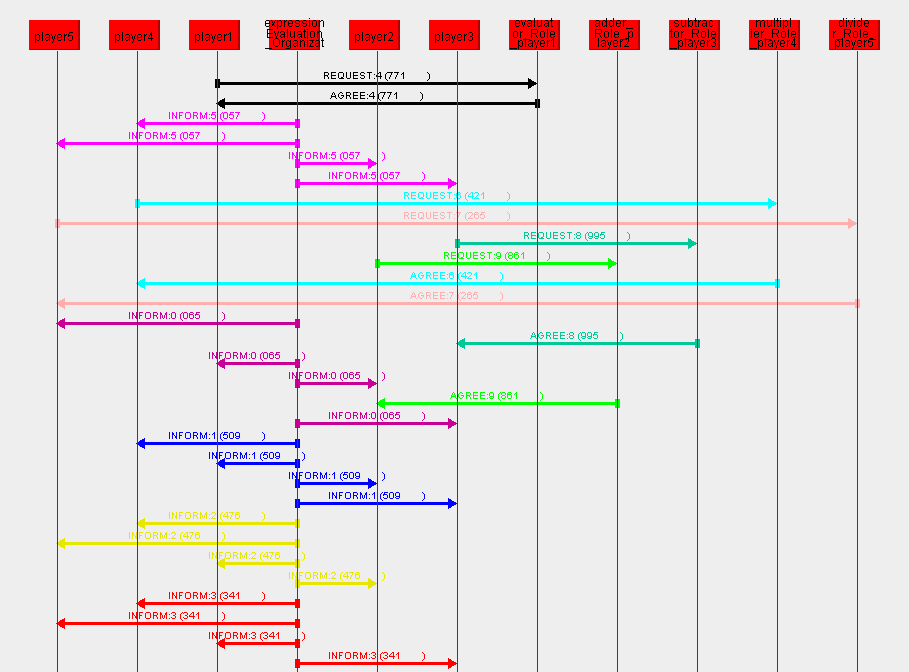
\includegraphics[width=\textwidth]{images/examples/example2-stage2.png}
	\caption{Stage 2: Role activation}
	\label{figure:example2-stage2}
\end{figure}

% Black
In the {\color{black}{\textbf{black}}} interaction scenario, \textit{player1} activates its \textit{Evaluator} role.
% Magenta
In the {\color{magenta}{\textbf{magenta}}} interaction scenario, the \textit{expression-evaluation} organization publishes the \textit{Role activated} event (for the \textit{Eveluator} role).
\textit{player2} reacts by activating its \textit{Adder} role (the {\color{green}{\textbf{green}}} interaction scenario), \textit{player3} by activating its \textit{Subtractor} role (the {\color{teal}{\textbf{teal}}} interaction scenario), \textit{player4} by activating its \textit{Multiplier} role (the {\color{cyan}{\textbf{cyan}}} interaction scenario) and \textit{player5} by activating its \textit{Divider} role (the {\color{pink}{\textbf{pink}}} interaction scenario).

% Green
In the {\color{green}{\textbf{green}}} interaction scenario, \textit{player2} activates its \textit{Adder} role.
% Red
In the {\color{red}{\textbf{red}}} interaction scenario, the \textit{expression-evaluation} organization publishes the \textit{Role activated} event (for the \textit{Adder} role).

% Teal
In the {\color{teal}{\textbf{teal}}} interaction scenario, \textit{player3} activates its \textit{Subtractor} role.
% Yellow
In the {\color{yellow}{\textbf{yellow}}} interaction scenario, the \textit{expression-evaluation} organization publishes the \textit{Role activated} event (for the \textit{Subtractor} role).

% Cyan
In the {\color{cyan}{\textbf{cyan}}} interaction scenario, \textit{player4} activates its \textit{Multiplier} role.
% Purple
In the {\color{purple}{\textbf{purple}}} interaction scenario, the \textit{expression-evaluation} organization publishes the \textit{Role activated} event (for the \textit{Multiplier} role).

% Pink
In the {\color{pink}{\textbf{pink}}} interaction scenario, \textit{player5} activates its \textit{Divider} role.
% Blue
In the {\color{blue}{\textbf{blue}}} interaction scenario, the \textit{expression-evaluation} organization publishes the \textit{Role activated} event (for the \textit{Divider} role).

% Event originator not notified
Note that that in all role activation scenarios, the player activating a role is not notified about the resulting \textit{Role activated} event, although it is subscribed to it; there is no need to notify the player causing the event in the first place.

%%%%%%%%%%%%%%%%%%%%%%%%%%%%%%%%%%%%%%%%%%%%%%%%%%%%%%%%%%%%%%%%%%%%%%%%%%%%%%%%
\subsubsection*{Stage 3: Competence and Responsibility Invocation}

% Figure: Stage 3: Competence and responsiility invocation
\begin{figure}[H]
	\centering
	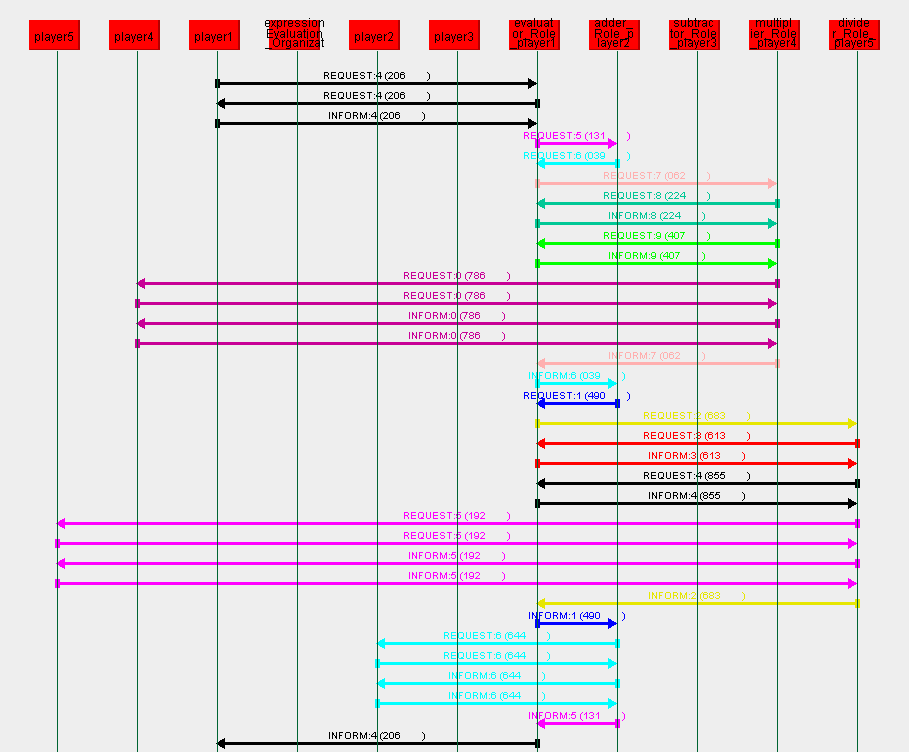
\includegraphics[width=\textwidth]{images/examples/example2-stage3.png}
	\caption{Stage 3: Competence and responsibility invocation}
	\label{figure:example2-stage3}
\end{figure}

The \textit{Evaluate expression} competence is invoked by \textit{player1} on its \textit{Evaluator} role and is carried out in a divide-and-conquer fashion by an \textit{Evaluator}, an \textit{Adder}, a \textit{Multiplier} and a \textit{Divider} by collaborating with one another and invoking responsibilities on their respective players.
In this example the arithmetic expression to be evaluated is $(1\cdot2)+(4/2)$.

% Evaluator: "(1*2)+(4/2)"
In the {\color{black}{\textbf{first black}}} interaction scenario, the \textit{evaluator-player1} position is requested by \textit{player1} to invoke the \textit{Evaluate} competence for the expression $(1\cdot2)+(4/2)$.
First, it parses the expression, finds the operation to be applied last---addition---and splits the expression into two sub-expressions to be added.
Next, it requests \textit{adder-player2} to evaluate their sum (the {\color{magenta}{\textbf{first magenta}}} interaction scenario).
Finally, it reports the value (4) to \textit{player1}.

% Adder: "(1*2)", "(4/2)"
In the {\color{magenta}{\textbf{first magenta}}} interaction scenario, the \textit{adder-player2} position is requested to evaluate the sum of the expressions $(1\cdot2)$ and $(4/2)$.
First, it requests \textit{evaluator-player1} to evaluate both expressions (the {\color{cyan}{\textbf{first cyan}}} and {\color{blue}{\textbf{blue}}} interaction scenarios).
Next, it invokes the \textit{Add} responsibility on \textit{player2} to calculate the sum of their values (the {\color{cyan}{\textbf{second cyan}}} interaction scenario).
Finally, it reports the sum (4) to \textit{evaluator-player1} (the original {\color{magenta}{\textbf{first magenta}}} interaction scenario).

% Evaluator: "(1*2)"
In the {\color{cyan}{\textbf{first cyan}}} interaction scenario, the \textit{evaluator-player1} position is requested to evaluate the expression $(1\cdot2)$.
First, it parses the expression, finds the last-to-be-applied operation---multiplication---and splits the expression into two sub-expressions to be multiplied.
Next, it requests \textit{multiplier-player4} to evaluate their product (the {\color{pink}{\textbf{pink}}} interaction scenario).
Finally, it reports the value (2) to \textit{adder-player2}.

% Multiplier: "1", "2"
In the {\color{pink}{\textbf{pink}}} interaction scenario, the \textit{multiplier-player4} position is requested to evaluate the product of the expressions $1$ and $2$.
First, it requests \textit{evaluator-player1} to evaluate both expressions (the {\color{teal}{\textbf{teal}}} and {\color{green}{\textbf{green}}} interaction scenarios).
Next, it invokes the \textit{Multiply} responsibility on \textit{player4} to calculate the product of their values (the {\color{purple}{\textbf{purple}}} interaction scenario).
Finally, it reports the product (2) to \textit{evaluator-player1} (the original {\color{pink}{\textbf{pink}}} interaction scenario).

% Evaluator: "1"
In {\color{teal}{\textbf{teal}}} interaction scenario, the \textit{evaluator-player1} is requested to evaluate the expression $1$.
It parses the expression, finds out it is a number (bottom case) and reports the value (1) to \textit{multiplier-player4}.

% Evaluator: "2"
In {\color{green}{\textbf{green}}} interaction scenario, the \textit{evaluator-player1} is requested to evaluate the expression $2$.
It parses the expression, finds out it is a number (bottom case) and reports the value (2) to \textit{multiplier-player4}.

% Evaluator: "(4/2)"
In the {\color{blue}{\textbf{blue}}} interaction scenario, the \textit{evaluator-player1} is requested to evaluate the expression $(4/2)$.
First, it parses the expression, finds the last-to-be-applied operation---division---and splits the expression into two sub-expressions to be divided.
Next, it requests \textit{divider-player5} to evaluate their product (the {\color{yellow}{\textbf{yellow}}} interaction scenario).
Finally, it reports the value (2) to \textit{adder-player2}.

% Divider: "4", "2"
In the {\color{yellow}{\textbf{yellow}}} interaction scenario, the \textit{divider-player5} position is requested to evaluate the quotient of the expressions $4$ and $2$.
First, it requests \textit{evaluator-player1} to evaluate both expressions (the {\color{red}{\textbf{red}}} and {\color{black}{\textbf{black}}} interaction scenarios).
Next, it invokes the \textit{Divide} responsibility on \textit{player5} to calculate the quotient of their values (the {\color{magenta}{\textbf{second magenta}}} interaction scenario).
Finally, it reports the quotient (2) to \textit{evaluator-player1} (the original {\color{yellow}{\textbf{yellow}}} interaction scenario).

% Evaluator: "4"
In {\color{red}{\textbf{red}}} interaction scenario, the \textit{evaluator-player1} is requested to evaluate the expression $4$.
It parses the expression, finds out it is a number (bottom case) and reports the value (4) to \textit{divider-player5}.

% Evaluator: "2"
In {\color{black}{\textbf{black}}} interaction scenario, the \textit{evaluator-player1} is requested to evaluate the expression $2$.
It parses the expression, finds out it is a number (bottom case) and reports the value (2) to \textit{divider-player5}.

%%%%%%%%%%%%%%%%%%%%%%%%%%%%%%%%%%%%%%%%%%%%%%%%%%%%%%%%%%%%%%%%%%%%%%%%%%%%%%%%
\subsubsection*{Stage 4: Role Deactivation}

% Figure: Stage 4: Role deactivation
\begin{figure}[H]
	\centering
	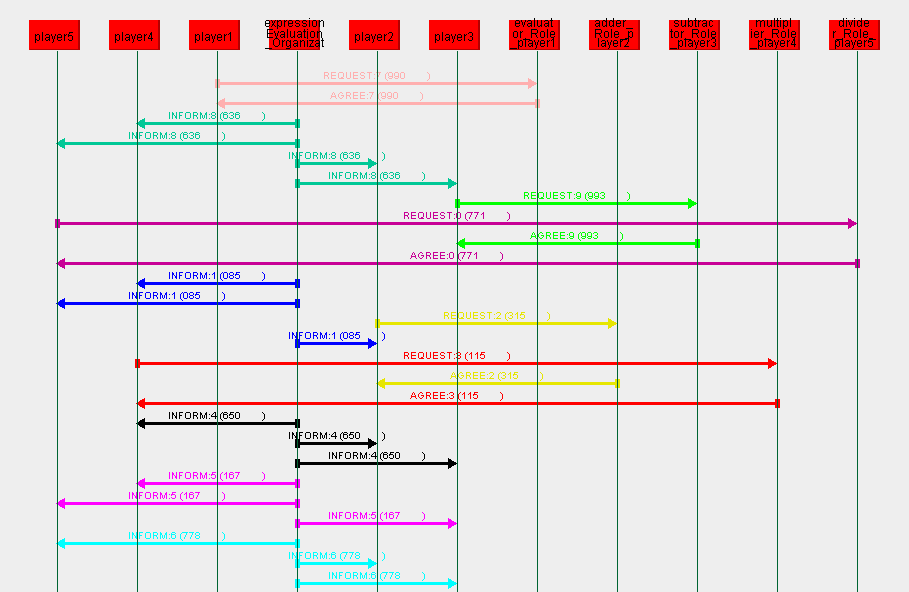
\includegraphics[width=\textwidth]{images/examples/example2-stage4.png}
	\caption{Stage 4: Role deactivation}
	\label{figure:example2-stage4}
\end{figure}

% Pink
In the {\color{pink}{\textbf{pink}}} interaction scenario, \textit{player1} deactivates its \textit{Evaluator} role.
% Teal
In the {\color{teal}{\textbf{teal}}} interaction scenario, the \textit{expression-evaluation} organization publishes the \textit{Role deactivated} event (for the \textit{Evaluator} role).
\textit{player2} reacts by deactivating its \textit{Adder} role (the {\color{yellow}{\textbf{yellow}}} interaction scenario), \textit{player3} by deactivating its \textit{Subtractor} role (the {\color{green}{\textbf{green}}} interaction scenario), \textit{player4} by deactivating its \textit{Multiplier} role (the {\color{red}{\textbf{red}}} interaction scenario) and \textit{player5} by deactivating its \textit{Divider} role (the {\color{purple}{\textbf{purple}}} interaction scenario).

% Yellow
In the {\color{yellow}{\textbf{yellow}}} interaction scenario, \textit{player2} deactivates its \textit{Adder} role.
% Magenta
In the {\color{magenta}{\textbf{magenta}}} interaction scenario, the \textit{expression-evaluation} organization publishes the \textit{Role deactivated} event (for the \textit{Adder} role).

% Green
In the {\color{green}{\textbf{green}}} interaction scenario, \textit{player3} deactivates its \textit{Subtractor} role.
% Blue
In the {\color{blue}{\textbf{blue}}} interaction scenario, the \textit{expression-evaluation} organization publishes the \textit{Role deactivated} event (for the \textit{Subtractor} role).

% Red
In the {\color{red}{\textbf{red}}} interaction scenario, \textit{player4} deactivates its \textit{Multiplier} role.
% Cyan
In the {\color{cyan}{\textbf{cyan}}} interaction scenario, the \textit{expression-evaluation} organization publishes the \textit{Role deactivated} event (for the \textit{Multiplier} role).

% Purple
In the {\color{purple}{\textbf{purple}}} interaction scenario, \textit{player5} deactivates its \textit{Divider} role.
% Black
In the {\color{black}{\textbf{black}}} interaction scenario, the \textit{expression-evaluation} organization publishes the \textit{Role deactivated} event (for the \textit{Divider} role).

%%%%%%%%%%%%%%%%%%%%%%%%%%%%%%%%%%%%%%%%%%%%%%%%%%%%%%%%%%%%%%%%%%%%%%%%%%%%%%%%
\subsubsection*{Stage 5: Role Deactment}

% Figure: Stage 5: Role deactment
\begin{figure}[H]
	\centering
	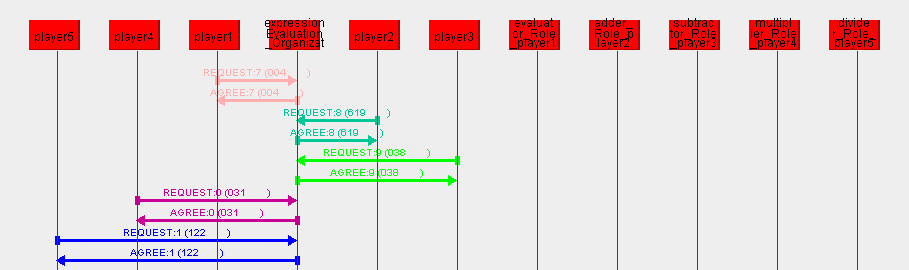
\includegraphics[width=\textwidth]{images/examples/example2-stage5.png}
	\caption{Stage 5: Role deactment}
	\label{figure:example2-stage5}
\end{figure} 

% Pink
In the {\color{pink}{\textbf{pink}}} interaction scenario, \textit{player1} deacts its \textit{Evaluator} role and the \textit{evaluator-player1} position is abolished.

% Teal
In the {\color{teal}{\textbf{teal}}} interaction scenario, \textit{player2} deacts its \textit{Adder} role and the \textit{adder-player2} position is abolished.

% Green
In the {\color{green}{\textbf{green}}} interaction scenario, \textit{player3} deacts its \textit{Subtractor} role and the \textit{subtractor-player3} position is abolished.

% Purple
In the {\color{purple}{\textbf{purple}}} interaction scenario, \textit{player4} deacts its \textit{Multiplier} role and the \textit{multiplier-player4} position is abolished.

% Blue
In the {\color{blue}{\textbf{blue}}} interaction scenario, \textit{player5} deacts its \textit{Divider} role and the \textit{divider-player5} position is abolished.